\documentclass[12pt,a4paper]{report}
\usepackage[english]{babel}
\usepackage{newlfont}
\usepackage{physics}
\usepackage{amsmath}
\usepackage{amssymb}
\usepackage{amsthm}
\usepackage{xcolor}
\usepackage{listings}
\usepackage{tikz}

\usetikzlibrary{quantikz}

\theoremstyle{definition}
\newtheorem{definition}{Definition}[section]

\theoremstyle{definition}
\newtheorem{example}{Example}[section]

\theoremstyle{definition}
\newtheorem{problem}{Problem}[section]

\textwidth=450pt\oddsidemargin=0pt
\newenvironment{dedication}
{%\clearpage           % we want a new page          %% I commented this
\thispagestyle{empty}% no header and footer
\vspace*{\stretch{1}}% some space at the top
\itshape             % the text is in italics
\raggedleft          % flush to the right margin
}
{\par % end the paragraph
\vspace{\stretch{3}} % space at bottom is three times that at the top
\clearpage           % finish off the page
}

\lstset{% This applies to ALL lstlisting
  basicstyle=\small\ttfamily\color{black},%
  breaklines=true,%
  numbers=none,
  moredelim=[s][\color{green!50!black}\ttfamily]{'}{'},% single quotes in green
}%







\begin{document}
\begin{titlepage}
\begin{center}
{{\Large{\textsc{Alma Mater Studiorum $\cdot$ Universit\`a di
Bologna}}}} \rule[0.1cm]{15.8cm}{0.1mm}
\rule[0.5cm]{15.8cm}{0.6mm}
{\small{\bf SCUOLA DI SCIENZE\\
Corso di Laurea in Informatica }}
\end{center}
\vspace{15mm}
\begin{center}
{\LARGE{\bf Static Analysis of Resources in QASM:}}\\
\vspace{3mm}
{\LARGE{\bf Estimation of the Number of Qubits}}\\
\end{center}
\vspace{40mm}
\par
\noindent
\begin{minipage}[t]{0.47\textwidth}
{\large{\bf Relatore:\\
Chiar.mo Prof.\\
Ugo Dal Lago\\
}}
\end{minipage}
\hfill
\begin{minipage}[t]{0.47\textwidth}\raggedleft
{\large{\bf Presentata da:\\
Damiano Scevola}}
\end{minipage}
\vspace{20mm}
\begin{center}
{\large{\bf Sessione I\\%inserire il numero della sessione in cui ci si laurea
Anno Accademico 2020/2021}}%inserire l'anno accademico a cui si è iscritti
\end{center}
\end{titlepage}

\begin{dedication}
A nonno Francesco
\end{dedication}

\tableofcontents



\chapter{Introduction}
The idea of quantum computing was conceived in the 1970s, when researchers of the caliber of Feynman, Manin and Deustch started to theorize that the properties of quantum mechanics might prove useful for performing computations differently from the classical paradigm. The main concept that lays at the core of this new model is the superposition of states, that is the simultaneous co-existence of multiple computational states at the same moment, with the possibility to perform the same operation to all of those states with a single computational step. Physical devices that are capable of such power are called ``quantum computers'', and they constitute a polynomial-time implementation of non-determinism, thus achieving an exponential-order level of parallelism. This fact invalidates the assumption that some problems (NP-complete ones, for instance) require too much time to be solved compared to human life duration, hence it opens the doors to a new variety of applications, and it also tears down the ones which rely on this assumption (like RSA cryptography). Literature usually refers to this scenario as ``Quantum Supremacy''.\\
Quantum computers operate through qubits, which are the quantum equivalent of bits, and can have not only $0$s and $1$s as values, but also combinations of them. Qubits are sequenced together to form quantum registers, which hold the actual computational power of quantum computers. For instance, a 3-qubit register can be in a superposition of the states $\ket{000}, \ket{001}, \ket{010}, \ldots, \ket{111}$, that are $2^3=8$ base states. Generalizing the previous result, we notice that an $n$-qubit register can represent up to $2^n$ states simultaneously, thus showing where the exponential speedup resides.\\
Some companies like Google and IBM have already built fully-functional quantum computers. However, all of them have a limited number of qubits due to the elevate cost of implementing them physically. Therefore, it is crucial that quantum programmers are thrifty with the usage of qubits while designing quantum circuits. The aim of this document is to show a simple tool which is able to analyze programs written in QASM language (Quantum Assembly) and check whether the number of qubits that are \textit{effectively} used is bounded by a certain expression.
We start by introducing some concepts of quantum computing, then we describe the QASM language and we provide details about the features that are taken into account by the analyzer. Then we proceed by going through the concepts of static analysis and symbolic execution, and finally we describe the tool that performs the estimation of the number of qubits.\\



\chapter{Quantum Computing}


\section{Quantum states}
\subsection{Deterministic systems}
In classical systems, when we need to encode the state of an object, we often use numbers. For example, consider a simple case where we have a skyscraper with $n$ floors (counting the ground floor also), and we want to represent on which one an employee is located. Trivially, this can be done using an integer number $k$, and if we assume there are no underground floors, then we can state $k \in \{0, 1, \ldots, n-1\}$.\\
Another option for representing such a state would be using a \textit{state vector}, that is a vector $\mathbf{v}\in\{0,1\}^n$ whose entries are all zeros except for the $k$-th, which is a $1$.
\begin{center}
\begin{tikzpicture}
\draw (0,0) -- (0,-6);
\draw (8,0) -- (8,-6);

\filldraw[black] (0,0) circle (2pt) node[anchor=west] {$n-1$};
\filldraw[black] (0,-1) circle (2pt) node[anchor=west] {$n-2$};
\filldraw[black] (0,-2) circle (0pt) node[anchor=west] {$\vdots$};
\filldraw[black] (0,-3) circle (3pt) node[anchor=west] {$k$};
\filldraw[black] (0,-4) circle (0pt) node[anchor=west] {$\vdots$};
\filldraw[black] (0,-5) circle (2pt) node[anchor=west] {$1$};
\filldraw[black] (0,-6) circle (2pt) node[anchor=west] {$0$};

\filldraw[black] (8,-0) circle (2pt) node[anchor=west] {$0$};
\filldraw[black] (8,-1) circle (2pt) node[anchor=west] {$0$};
\filldraw[black] (8,-2) circle (0pt) node[anchor=west] {$\vdots$};
\filldraw[black] (8,-3) circle (3pt) node[anchor=west] {$1$};
\filldraw[black] (8,-4) circle (0pt) node[anchor=west] {$\vdots$};
\filldraw[black] (8,-5) circle (2pt) node[anchor=west] {$0$};
\filldraw[black] (8,-6) circle (2pt) node[anchor=west] {$0$};
\end{tikzpicture}
\end{center}
Such an approach seems exaggerated for this simple case, but it is crucial to understand how quantum systems work. Let's take a look at another scenario.




\subsection{Probabilistic systems}
Imagine now that the floor the employee is on is not known for sure, but we are only given probabilities of her being on each floor. The state vector now looks something like:
\begin{equation*}
    \mathbf{v}=\begin{bmatrix}
        p_0\\
        p_1\\
        \vdots\\
        p_{n-1}\\
    \end{bmatrix}\in [0,1]^n
\end{equation*}
We now have a generalized version of our previously defined state vector, because each entry $p_i$ is a real number between $0$ and $1$. Since we are talking about probabilities, we set the constraint that all the entries of $\mathbf{v}$ must sum up to $1$.
\begin{equation*}
    \sum_{i=0}^{n-1} p_i = 1
\end{equation*}
It should be noticed that there is no way to represent probabilistic states with a single number like we do for deterministic ones. It is clear, however, that in case we know the exact location of the employee, the vector would collapse to the previous case. In fact, if we are certain that the employee is on the $k$-th floor, then $p_k=1$, and $\forall i \in \{0,1,\ldots,n-1\} \smallsetminus \{k\},\ p_i=0$.\\
Now it is time to define state vectors for quantum systems.\\




\subsection{Quantum systems}
Consider a quantum object (e.g. an electron or a photon), and assume its position can be measured in the domain $\{x_1, x_2, \ldots, x_n\}$.\\
\begin{center}
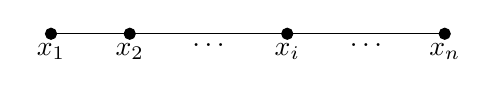
\begin{tikzpicture}
\draw (0,0) -- (5,0);
\filldraw[black] (0,0) circle (2pt) node[anchor=north] {$x_1$};
\filldraw[black] (1,0) circle (2pt) node[anchor=north] {$x_2$};
\filldraw[black] (2,0) circle (0pt) node[anchor=north] {$\ldots$};
\filldraw[black] (3,0) circle (2pt) node[anchor=north] {$x_i$};
\filldraw[black] (4,0) circle (0pt) node[anchor=north] {$\ldots$};
\filldraw[black] (5,0) circle (2pt) node[anchor=north] {$x_n$};
\end{tikzpicture}
\end{center}

To each position $x_i$, it corresponds a basic vector having as entries all zeros and a $1$ as the $i$-th entry.
\begin{equation*}
    \ket{x_1} = \begin{bmatrix}
        1\\
        0\\
        \vdots\\
        0\\
    \end{bmatrix},\ 
    \ket{x_2} = \begin{bmatrix}
        0\\
        1\\
        \vdots\\
        0\\
    \end{bmatrix},\ \ldots,\ 
    \ket{x_n} = \begin{bmatrix}
        0\\
        0\\
        \vdots\\
        1\\
    \end{bmatrix}
\end{equation*}

\begin{definition}[Quantum State]
A quantum state $\ket{\psi}$ is a linear combination of the basic vectors $\ket{x_1}, \ket{x_2}, \ldots, \ket{x_n}$ having complex weights $c_1, c_2, \ldots, c_n \in \mathbb{C}$.
\begin{equation*}
    \ket{\psi}=c_1\ket{x_1}+c_2\ket{x_2}+\cdots+c_n\ket{x_n}
\end{equation*}
Therefore, $\ket{\psi}$ can be represented as
\begin{equation*}
    \ket{\psi}=\begin{bmatrix}
        c_0\\
        c_1\\
        \vdots\\
        c_{n-1}\\
    \end{bmatrix}\in \mathbb{C}^n
\end{equation*}
where
\begin{equation*}
    \sum_{i=0}^{n-1} \left\lvert c_i \right\rvert ^2 = 1
\end{equation*}
\end{definition}
Since it is a weighted sum of basic states, we say that $\ket{\psi}$ is a \textit{superposition} of the basic states.
The square norm of $c_i$ tells us the probability of observing the particle in the position $x_i$, and since the particle is indeed in one of those positions, the sum of square norms must add up to $1$.\\
The reason why we need complex numbers to represent quantum states is that quantum objects (like photons or electrons) behave both like particles and waves, so they can interfere either constructively or disruptively. By using complex numbers, we can sum waves and capture the fact that they could interfere disruptively, since the square norm of the sum of two complex number is not necessarily greater than both of the square norms of the addends.



\section{Qubits and quantum registers}
\subsection{Bits and qubits}
In order to understand what qubits are, we should remark the meaning of classical bits and then make a generalization.
\begin{definition}[Bit]
A bit is an elementary unit of information describing the state of the simplest classical system.
\end{definition}
As we know, a bit can only assume values in the domain $\{0,1\}$.
\begin{center}
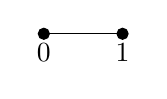
\begin{tikzpicture}
\draw (0,0) -- (1,0);
\filldraw[black] (0,0) circle (2pt) node[anchor=north] {$0$};
\filldraw[black] (1,0) circle (2pt) node[anchor=north] {$1$};
\end{tikzpicture}
\end{center}
By following the approach of the previous section, we can also describe bits using a two-dimensional state vector, where the first element stands for $0$, and the last for $1$:
\begin{equation*}
    \ket{0}=\begin{bmatrix}
        1\\
        0
    \end{bmatrix},\ 
    \ket{1}=\begin{bmatrix}
        0\\
        1
    \end{bmatrix}
\end{equation*}
If we take $\ket{0}$ and $\ket{1}$ as basic states, we can define a quantum system by considering all normalized linear combinations of those states. Such a quantum system is called \textit{qubit}.
\begin{definition}[Qubit]
A qubit is a quantum system having $\ket{0}$ and $\ket{1}$ as basic states, and therefore it can be represented as an element of $\mathbb{C}^2$.
\begin{equation*}
    \ket{q}=c_0\ket{0}+c_1\ket{1}=c_0\begin{bmatrix}
        1\\
        0
    \end{bmatrix}+c_1\begin{bmatrix}
        0\\
        1
    \end{bmatrix}=\begin{bmatrix}
        c_0\\
        c_1
    \end{bmatrix} \in \mathbb{C}^2
\end{equation*}
Keep in mind that the sum of the square norms must be equal to $1$. In other words, the state must be \textit{normalized}.
\begin{equation*}
    \left|c_0\right|^2+\left|c_1\right|^2=1
\end{equation*}
\end{definition}
\begin{example}
Here is an example of a qubit:
\begin{equation*}
    \ket{q}=\frac{\ket{0}+\ket{1}}{\sqrt{2}}=\begin{bmatrix}
        \frac{1}{\sqrt{2}}\\
        \frac{1}{\sqrt{2}}
    \end{bmatrix}
\end{equation*}
In fact, if we check the sum of the square norms of the coefficients, we see that they add up to $1$.
\begin{equation*}
    \left(\frac{1}{\sqrt{2}}\right)^2+\left(\frac{1}{\sqrt{2}}\right)^2=\frac{1}{2}+\frac{1}{2}=1
\end{equation*}
Of course, the following are also qubits:
\begin{equation*}
    \ket{q_0}=\frac{\ket{0}-\ket{1}}{\sqrt{2}}=\begin{bmatrix}
        \frac{1}{\sqrt{2}}\\
        -\frac{1}{\sqrt{2}}
    \end{bmatrix},\ 
    \ket{q_1}=\frac{\ket{1}-\ket{0}}{\sqrt{2}}=\begin{bmatrix}
        -\frac{1}{\sqrt{2}}\\
        \frac{1}{\sqrt{2}}
    \end{bmatrix}
\end{equation*}
\end{example}
We shall notice that $\ket{q}$, $\ket{q_0}$ and $\ket{q_1}$ are all superpositions of the basic states $\ket{0}$ and $\ket{1}$.




\subsection{Measurement}
When we measure a qubit, the possible outcomes are only $0$ and $1$, and the probability of observing the one or the other is dictated by the square norms of the coefficients $c_0$ and $c_1$. In addition to this, the measurement affects the internal state of the qubit permanently, making it collapse to the value that has just been measured.
\begin{example}
Consider a qubit whose state is
\begin{equation*}
    \ket{\psi}=\frac{\sqrt{3}}{2}\ket{0}+\frac{1}{2}\ket{1}
\end{equation*}
If we measure it, we have $\left(\frac{\sqrt{3}}{2}\right)^2=\frac{3}{4}=75\%$ of probability to observe the outcome being $0$, and $\left(\frac{1}{2}\right)^2=\frac{1}{4}=25\%$ of probability of it being $1$.\\
Let's say we obtained $0$ from the measurement. The state of the qubit is not $\ket{\psi}$ anymore, but it has become $\ket{\psi'}=\ket{0}$ because the measurement made it collapse as a side effect, so if we measure it again we have $100\%$ of chances to observe the value $0$ again.\\
This fact is at the core of quantum mechanics, and it just tells us that in order to observe something we must inevitably interact with it and alter its internal state.
\end{example}




\subsection{Quantum registers}
Quantum computers with a single qubit are not very interesting, so we need a way to combine qubits and form registers. In order to combine quantum systems, we need to use the tensor product.
For example, let's say we wanted to represent the two-qubits state $\ket{01}$. We would then need to compute the tensor product $\ket{0}\otimes\ket{1}$ as follows:
\begin{equation*}
    \ket{0}\otimes\ket{1}=\begin{bmatrix}
        1\\
        0
    \end{bmatrix}\otimes\begin{bmatrix}
        0\\
        1
    \end{bmatrix}=\begin{bmatrix}
        1\begin{bmatrix}
            0\\
            1
        \end{bmatrix}\\
        0\begin{bmatrix}
            0\\
            1
        \end{bmatrix}
    \end{bmatrix}=\begin{bmatrix}
            0\\
            1\\
            0\\
            0
    \end{bmatrix}=\begin{bmatrix}
            c_{00}\\
            c_{01}\\
            c_{10}\\
            c_{11}
    \end{bmatrix}
\end{equation*}
If we observe the result carefully, we can notice that the normalization constraint still holds, and the only $1$ that appears in the final result corresponds to $c_{01}$, which is right the coefficient labelled with our state $\ket{01}$. If we try to do the same thing with the state $\ket{101}$, we will obtain:
\begin{equation*}
    \ket{101}=\ket{1}\otimes\ket{0}\otimes\ket{1}=\begin{bmatrix}
        0\\
        0\\
        0\\
        0\\
        0\\
        1\\
        0\\
        0
    \end{bmatrix}=\begin{bmatrix}
        c_{000}\\
        c_{001}\\
        c_{010}\\
        c_{011}\\
        c_{100}\\
        c_{101}\\
        c_{110}\\
        c_{111}
    \end{bmatrix}
\end{equation*}
Since the result of the tensor product enumerates all possible states with $n$ qubits, the dimension of the output is as large as $2^n$.\\
Of course, considering the fact that quantum computers allow superpositions of many states, we shall clarify that the previous examples have only taken into account basic states. Hence we can also have a 3-qubit register in the state
\begin{equation*}
    \ket{\psi}=\frac{\ket{000}+\ket{010}-\ket{011}-\ket{100}+\ket{110}}{\sqrt{5}}
\end{equation*}



\subsection{Entanglement}
When multiple qubits are involved to form a quantum register, it can sometimes have the property that if we measure one of the qubits, then we automatically know the value of the others. We say, then, that those qubits are \textit{entangled}.
\begin{example}
Consider a quantum register with 2 qubits and assume its state is
\begin{equation*}
    \ket{\psi}=\frac{\ket{00}+\ket{11}}{\sqrt{2}}
\end{equation*}
Then, if we measure the first qubit and we observe the value $1$, we automatically know that the other qubit also has value $1$ by just noticing that the only basic state that appears in $\ket{\psi}$ and has a $\ket{1}$ at the first position is $\ket{11}$, so we know for sure that the other one is $\ket{1}$ too.\\
In this case, the measurement not only affects the state of the measured qubit making it collapse to $\ket{1}$, but it also collapses the state of the entangled one.
\end{example}




\section{Quantum Gates}
So far we have discussed how to represent qubits and quantum registers and what their properties are, but in order to perform a computation we need a way to manipulate them according to an algorithm and exploit their computational power.\\
Just like classical computers manipulate bits using logic gates, quantum computers use quantum gates to achieve their objective.\\
The physical implementation of quantum gates is as complicated as that of qubits, but we can represent what these gates do by using mathematical objects that operate on state vectors and keep the output normalized so that the sum of the square norms of the coefficients of the output vector is always $1$. These objects are unitary matrices.\\
There are infinite possible quantum gates. Here we describe the set of universal ones $\{H, CNOT, R(\theta)\}$, which includes three gates that can be combined together to simulate an arbitrary gate.\\




\subsection{Hadamard gate}
The Hadamard gate is encoded by the following matrix:
\begin{equation*}
    H=\begin{bmatrix}
        \frac{1}{\sqrt{2}} & \frac{1}{\sqrt{2}} \\
        \frac{1}{\sqrt{2}} & -\frac{1}{\sqrt{2}} \\
    \end{bmatrix}=\frac{1}{\sqrt{2}}\begin{bmatrix}
        1 & 1 \\
        1 & -1
    \end{bmatrix}
\end{equation*}
The Hadamard matrix is the transition matrix from the canonical basis $\left\{\begin{bmatrix} 1 \\ 0\end{bmatrix}, \begin{bmatrix} 0 \\ 1\end{bmatrix}\right\}$ to the Hadamard basis $\left\{\begin{bmatrix} \frac{1}{\sqrt{2}} \\ \frac{1}{\sqrt{2}}\end{bmatrix}, \begin{bmatrix} \frac{1}{\sqrt{2}} \\ -\frac{1}{\sqrt{2}}\end{bmatrix}\right\}$, which is used to express arbitrary states in terms of superpositions of basic states, and this allows calculations to be performed on a superposition, hence on all of the basic states it is composed of with a single computational step.\\
Since $H$ is unitary, by applying it twice we go back to the canonical basis, so after calculations are finished, Hadamard gate can be applied again to translate the results back into the canonical basis, ready to be measured by the observer.
\begin{example}
By applying Hadamard gate to the qubits $\ket{0}$ and $\ket{1}$ we get:
\begin{equation*}
    H\ket{0}=\begin{bmatrix}
        \frac{1}{\sqrt{2}} & \frac{1}{\sqrt{2}} \\
        \frac{1}{\sqrt{2}} & -\frac{1}{\sqrt{2}}
    \end{bmatrix}\begin{bmatrix}
        1 \\
        0
    \end{bmatrix}=\begin{bmatrix}
        \frac{1}{\sqrt{2}} \\
        \frac{1}{\sqrt{2}}
    \end{bmatrix}=\frac{\ket{0}+\ket{1}}{\sqrt{2}}=\ket{+}
\end{equation*}
\begin{equation*}
    H\ket{1}=\begin{bmatrix}
        \frac{1}{\sqrt{2}} & \frac{1}{\sqrt{2}} \\
        \frac{1}{\sqrt{2}} & -\frac{1}{\sqrt{2}}
    \end{bmatrix}\begin{bmatrix}
        0 \\
        1
    \end{bmatrix}=\begin{bmatrix}
        \frac{1}{\sqrt{2}} \\
        -\frac{1}{\sqrt{2}}
    \end{bmatrix}=\frac{\ket{0}-\ket{1}}{\sqrt{2}}=\ket{-}
\end{equation*}
It is easy to verify that applying Hadamard on $\ket{+}$ and $\ket{-}$ we go back respectively to $\ket{0}$ and $\ket{1}$.\\
We will represent the Hadamard gate as a box labelled with `H'\\\\
\begin{quantikz}
    & \lstick{$\ket{0}$} & \gate{H} & \rstick{$\frac{\ket{0}+\ket{1}}{\sqrt{2}}$}\qw&\\
\end{quantikz}\\
\end{example}





\subsection{Controlled NOT gate}
While Hadamard gate affects a single qubit, the controlled NOT gate (CNOT or CX for short) needs two of them. One is the control qubit, and the other is the target.
\begin{quantikz}\\
\lstick{$\ket{x}$} & \ctrl{1} & \rstick{$\ket{x}$} \qw& \\
\lstick{$\ket{y}$} & \targ{} & \rstick{$\ket{x\oplus y}$} \qw& \\
\end{quantikz}\\
Here $\oplus $ denotes the binary exclusive OR operation. That is, if $\ket{x} = \ket{0}$ then the bottom output will be left unaltered, otherwise if $\ket{x} = \ket{1}$, then the bottom qubit is flipped.
The matrix that corresponds to the CNOT gate is:
\begin{equation*}
    \prescript{C}{}{X} = \begin{bmatrix}
    1 & 0 & 0 & 0\\
    0 & 1 & 0 & 0\\
    0 & 0 & 0 & 1\\
    0 & 0 & 1 & 0
    \end{bmatrix}
\end{equation*}




\subsection{Phase shift gate}
Phase shift gate is a parametric gate that affects a single qubit by rotating it in the Bloch sphere, adjusting its phase. We will not go over the details of Bloch sphere representation, but we just give the matrix which encodes the phase shift here.
\begin{equation*}
    R(\theta) = \begin{bmatrix}
        1 & 0 \\
        0 & e^\theta
    \end{bmatrix}
\end{equation*}
Now that we have discussed quantum gates, we can move to designing quantum circuits (or algorithms).





\section{Quantum Circuits}
Quantum circuits are the equivalent of algorithms for classical computing. By combining quantum gates, we can build a circuit that performs a certain computation and exploits the power of superpositions to drastically reduce the time of execution compared to a classical program.
\begin{definition}[Quantum circuit] % CITE Qiskit
A quantum circuit is a computational routine consisting of coherent quantum operations on quantum data, such as qubits, and concurrent real-time classical computation. It is an ordered sequence of quantum gates, measurements and resets, all of which may be conditioned on and use data from the real-time classical computation.
\end{definition}
In order to understand how quantum circuits work, we will discuss the Deutsch algorithm for balanced and constant function classification.





\subsection{Deutsch algorithm}
Before describing the Deutsch algorithm, let's define what balanced and constant functions are.
\begin{definition}[Balanced and constant functions]
A function $f: \{0,1\} \longrightarrow \{0,1\}$ is \textit{balanced} if $f(0)\neq f(1)$, otherwise it is \textit{constant}.
\end{definition}
The Deutch algorithm solves the following problem:
\begin{problem}[Deutsch-Jozsa]
Suppose we have a function $f: \{0,1\} \longrightarrow \{0,1\}$ which we can evaluate, but we do not know its exact definition. Determine whether $f$ is balanced or constant.
\end{problem}
If we wanted to use the classical approach, we would need to evaluate $f$ twice and compare the results. With the Deutsch algorithm, we will see that only one evaluation is sufficient.\\
Suppose we have a unitary matrix $U_f$ that encodes $f$:\\
\begin{quantikz}\\
    & \lstick{$\ket{x}$} & \qw & \qw & \gate[wires=2][2cm]{U_f}& \qw & \qw & \rstick{$\ket{x}$}\qw\\
    & \lstick{$\ket{y}$} & \qw & \qw & & \qw & \qw & \rstick{$\ket{y \oplus f(x)}$}\qw\\
\end{quantikz}\\
Let's now build a circuit that uses $U_f$ and solves our problem:\\
\begin{quantikz}\\
    & \lstick{$\ket{0}$} & \qw & \gate{H} & \qw & \gate[wires=2][2cm]{U_f}& \qw & \gate{H} & \qw & \meter{}\\
    & \lstick{$\ket{1}$} & \qw & \gate{H} & \qw &  & \qw & \qw & \qw & \qw &\\
    & & \text{$\ket{\psi_0}$} &  & \text{$\ket{\psi_1}$}  &  & \text{$\ket{\psi_2}$} &  &   \text{$\ket{\psi_3}$} &  &\\
\end{quantikz}\\
In terms of matrices, the circuit corresponds to
\begin{equation*}
    (H \otimes I)U_f(H \otimes H)\ket{0,1}
\end{equation*}
The algorithm starts with the state
\begin{equation*}
    \ket{\psi_0} = \ket{0, 1}
\end{equation*}
Then it proceeds by applying Hadamard to both qubits, putting them in a superposition:
\begin{equation*}
    \ket{\psi_1} = \ket{+,-} = \left[\frac{\ket{0}+\ket{1}}{\sqrt{2}}\right]\left[\frac{\ket{0}-\ket{1}}{\sqrt{2}}\right]=\frac{\ket{0,0}-\ket{0,1}+\ket{1,0}-\ket{1,1}}{2}
\end{equation*}
Now let's pause for a moment and ponder about what happens if we apply $U_f$ to a generic state $\ket{x, -}$.
\begin{equation*}
    U_f\ket{x,-}=U_f(\ket{x}\left[\frac{\ket{0}-\ket{1}}{\sqrt{2}}\right])=U_f\left[\frac{\ket{x,0}-\ket{x,1}}{\sqrt{2}}\right]=\ket{x}\left[\frac{\ket{0 \oplus f(x)}-\ket{1 \oplus f(x)}}{\sqrt{2}}\right]
\end{equation*}
Which simplifies to
\begin{equation*}
    U_f\ket{x,-}=\ket{x}\left[\frac{\ket{f(x)}-\ket{\overline{f(x)}}}{\sqrt{2}}\right]
\end{equation*}
Where we denoted the opposite of $f(x)$ with $\overline{f(x)}$. So we have
\begin{equation*}
    U_f\ket{x,-}=\begin{cases}
        \ket{x}\left[\frac{\ket{0}-\ket{1}}{\sqrt{2}}\right] & if\ f(x) = 0\\
        \ket{x}\left[\frac{\ket{1}-\ket{0}}{\sqrt{2}}\right] & if\ f(x) = 1\\
    \end{cases}
\end{equation*}
We can write the last expression as
\begin{equation*}
    U_f\ket{x,-}=(-1)^{f(x)}\ket{x}\left[\frac{\ket{0}-\ket{1}}{\sqrt{2}}\right]=(-1)^{f(x)}\ket{x}\ket{-}
\end{equation*}
Going back to our circuit, this means that, after applying $U_f$ to $\ket{\psi_1}$, we get
\begin{align*}
    \ket{\psi_2}=U_f\ket{+,-}&=\frac{U_f\ket{0,-}+U_f\ket{1,-}}{\sqrt{2}}\\
    &=\frac{(-1)^{f(0)}\ket{0}+(-1)^{f(1)}\ket{1}}{\sqrt{2}}\ket{-}
\end{align*}
Now let's see what happens in the two cases where $f$ is balanced or it is constant.
If $f$ is balanced $f(0)\neq f(1)$, then the top qubit becomes either $\frac{\ket{0}-\ket{1}}{\sqrt{2}}$ or $\frac{-\ket{0}+\ket{1}}{\sqrt{2}}$ depending on which way it is balanced, but in either case we can write
\begin{equation*}
    \ket{\psi_2}=(\pm 1)\frac{\ket{0}-\ket{1}}{\sqrt{2}}\ket{-}=(\pm 1)\ket{-,-}
\end{equation*}
Since the coefficient $(\pm 1)$ is global, it can be ignored due to the normalization constraint, so we can say $\ket{\psi_2}=\ket{-,-}$ if $f$ is balanced.\\
On the other hand, if $f$ is constant $f(0)=f(1)$, then the top qubit becomes either $\frac{\ket{0}+\ket{1}}{\sqrt{2}}$ or $\frac{-\ket{0}-\ket{1}}{\sqrt{2}}$, but in either case we can write
\begin{equation*}
    \ket{\psi_2}=(\pm 1)\frac{\ket{0}+\ket{1}}{\sqrt{2}}\ket{-}=(\pm 1)\ket{+,-}
\end{equation*}
Here the argument for $(\pm 1)$ still holds, so we can say $\ket{\psi_2}=\ket{+,-}$ if f is constant.\\
Summing up, we have
\begin{equation*}
    \ket{\psi_2}=\begin{cases}
        \ket{+,-}\ if\ f\ is\ constant\\
        \ket{-,-}\ if\ f\ is\ balanced
    \end{cases}
\end{equation*}
Finally, the last Hadamard gate brings our state back to the canonical basis, and so
\begin{equation*}
    \ket{\psi_3} = \begin{cases}
        \ket{0,-}\ if\ f\ is\ constant\\
        \ket{1,-}\ if\ f\ is\ balanced
    \end{cases}
\end{equation*}
Now we can measure the top qubit, and we can be sure about the function being balanced or constant by just looking at the result.\\
Notice that the quantum algorithm only evaluated the function once, namely on the superposition $\ket{+,-}$. The generalized version of this algorithm, the Deutsch-Jozsa algorithm, shows the speedup in the computation even more.






\subsection{Deutsch-Jozsa algorithm}
Although we are not going to illustrate all the analysis of the Deutsch-Jozsa algorithm, we will still define the problem, show the circuit that solves it and state some facts about its computational complexity compared to the classical case.
Let's generalize the definition of balanced and constant functions.
\begin{definition}[Balanced and constant functions]
    A function $f: \{0,1\}^n \longrightarrow \{0,1\}$ is \textit{balanced} if exactly half of the inputs go to $0$ (and the other half go to $1$), while it is \textit{constant} if all of the inputs go to the same output (either $0$ or $1$).
\end{definition}
The Deutsch-Jozsa problem is the same as the Deutsch one, with the assumptions that $f:\{0,1\}^n\longrightarrow \{0,1\}$ and that $f$ is guaranteed to be either constant or balanced.\\
With the classical approach, in order to determine whether $f$ is balanced or constant we need to evaluate it at most on one plus half of the inputs. This is because as soon as we detect two different output values, we can conclude that the function is balanced, but if $f$ is constant, we cannot be sure of it until we check that more than half of its outputs are the same. So the worst case scenario requires $1 + \frac{2^n}{2} = 1 + 2^{n-1}$ evaluations, which is exponential with respect to the size of the input.\\
Let's now delve into the quantum world and contemplate its power.\\
Since we are given the possibility to evaluate $f$, assume there is a unitary matrix $U_f$ that fulfills the task:\\
\begin{quantikz}\\
    & \lstick{$\ket{\mathbf{x}}$} & \qw & \qwbundle{n}\qw & \gate[wires=2][2cm]{U_f}& \qw & \qwbundle{n}\qw & \rstick{$\ket{\mathbf{x}}$}\qw\\
    & \lstick{$\ket{y}$} & \qw & \qw & & \qw & \qw & \rstick{$\ket{f(\mathbf{x})\oplus y}$}\qw\\
\end{quantikz}\\
Here we denoted the top input $\ket{\mathbf{x}}=\ket{x_0x_1\ldots x_{n-1}}$ in bold and the wire mark \begin{quantikz} & \qwbundle{n}\qw \end{quantikz} indicates that it is a bit sting with length $n$.
The circuit that solves the problem  is the following:\\
\begin{quantikz}\\
    & \lstick{$\ket{\mathbf{0}}$} & \qw & \qwbundle{n}\qw & \gate{H^{\otimes n}} & \qw & \qwbundle{n}\qw & \gate[wires=2][2cm]{U_f}& \qw & \qwbundle{n}\qw & \gate{H^{\otimes n}} & \qw & \qwbundle{n}\qw & \meter{}\\
    & \lstick{$\ket{1}$} & \qw & \qw & \gate{H} & \qw & \qw &  & \qw & \qw & \qw & \qw & \qw & \qw &\\
\end{quantikz}\\
We can notice that it is very similar to the Deutsch circuit, with the only difference that there are $n$ qubits as the top input, and we denoted the fact that we are applying Hadamard to each one of them with the gate $H^{\otimes n}$, that is the tensor product of $n$ Hadamard matrices.\\
This circuit is capable to tell us if $f$ is balanced or constant in a single run. In other words, we have an exponential speedup compared to the classical algorithm for the same problem. There are many other problems that benefit of the quantum speedup, and some of them are of a practical nature. This is why quantum computing is so powerful.\\
In order to design and execute quantum algorithms, we need a language that allows us to describe them in terms of gates and classical instructions. In the next chapter we will explore OpenQASM, which is a powerful and compact language that achieves the goal.









\chapter{OpenQASM}
% CITE OpenQASM
OpenQASM is an imperative programming language designed for quantum algorithms and applications. It has a dual nature as an assembly language and as a hardware description language. There are multiple versions of OpenQASM, but we will describe a simplified version of OpenQASM 3.0.\\
The formal grammar of the language is presented using the ANTLRv4 syntax, and starts with:
\begin{lstlisting}
program
    : header (globalStatement | statement)*
    ;
\end{lstlisting}
So we first describe the header and then we proceed to discuss the other aspects of the language, which also include statements. In each section we will present the formal grammar and comment it providing informal semantic and context.




\section{Header}
\begin{lstlisting}
header
    : version? include*
    ;

version
    : 'OPENQASM' (Integer | RealNumber) SEMICOLON
    ;

include
    : 'include' StringLiteral SEMICOLON
    ;
\end{lstlisting}
The header consists in an optional version string followed by zero or more `include' statements, that are used to import gates and functions from other files at compile time.\\
A typical example of what the header looks like is:
\begin{lstlisting}
// Header
OPENQASM 3.0;
/*
comment
*/
include "stdgates.qasm";
\end{lstlisting}
We can see here that comments are C-like, and string literals are wrapped by double quotes.\\
From now on we will proceed in a bottom-up fashion, describing all the features of the language that are used in more complex rules, starting from lexicon, types and index identifiers up to global and non-global statements.


\section{Lexer rules}
\begin{lstlisting}
LBRACKET: '[';
RBRACKET: ']';

LBRACE: '{';
RBRACE: '}';

LPAREN: '(';
RPAREN: ')';

COLON: ':';
SEMICOLON: ';';

DOT: '.';
COMMA: ',';

EQUALS: '=';
ARROW: '->';

PLUS: '+';
MINUS: '-';
MUL: '*';
DIV: '/';
MOD: '%';


Constant: ( 'pi' | 'tau' | 'euler' );

Whitespace: [ \t]+ -> skip;
Newline: [\r\n]+ -> skip;

fragment Digit: [0-9];
Integer: Digit+;

fragment ValidUnicode: [\p{Lu}\p{Ll}\p{Lt}\p{Lm}\p{Lo}\p{Nl}];
fragment Letter: [A-Za-z];
fragment FirstIdCharacter: '_' | '$' | ValidUnicode | Letter;
fragment GeneralIdCharacter: FirstIdCharacter | Integer;

Identifier: FirstIdCharacter GeneralIdCharacter*;

fragment SciNotation: [eE];
fragment PlusMinus: PLUS | MINUS;
fragment Float: Digit+ DOT Digit*;
RealNumber: Float (SciNotation PlusMinus? Integer)?;

LineComment: '//' ~[\r\n]* -> skip;
BlockComment: '/*' .*? '*/' -> skip;

StringLiteral
    : '"' ~["\r\t\n]+? '"'
    | '\'' ~['\r\t\n]+? '\''
    ;

\end{lstlisting}


\section{Types}
In OpenQASM, types are divided in two categories: quantum types and classical types.
\subsection{Quantum types}
\begin{lstlisting}
quantumType
    : 'qubit'
    | 'qreg'
    ;
\end{lstlisting}
We will describe how to make a quantum declaration in the `Global statements' section.

\subsection{Classical types}
\begin{lstlisting}
classicalType
    : singleDesignatorType designator
    | doubleDesignatorType doubleDesignator
    | noDesignatorType
    | bitType designator?
    ;

bitType
    : 'bit'
    | 'creg'
    ;

singleDesignatorType
    : 'int'
    | 'uint'
    | 'float'
    | 'angle'
    ;

doubleDesignatorType
    : 'fixed'
    ;

noDesignatorType
    : 'bool'
    ;

designator
    : LBRACKET expression RBRACKET
    ;

doubleDesignator
    : LBRACKET expression COMMA expression RBRACKET
    ;
\end{lstlisting}
A \texttt{designator} is simply a parameter for the type, for example \texttt{int[16]} indicates a 16-bit integer, where \texttt{16} is the designator. The single designator for the \texttt{float} and \texttt{angle} types is for specifying the precision. Another example could be \texttt{fixed[7, 24]}, which indicates a $24+7+1=32$-bit fixed point signed number having 7 integer bits and 24 fractional bits.\\
\texttt{bitType} has a single designator that stands for the number of bits of the  array (or register, equivalently), while only the boolean type has no designator.\\



\section{Index identifiers}
\begin{lstlisting}
indexIdentifier
    : Identifier rangeDefinition
    | Identifier (LBRACKET expressionList RBRACKET)?
    | indexIdentifier '||' indexIdentifier
    ;

indexIdentifierList
    : (indexIdentifier COMMA)* indexIdentifier
    ;

indexEqualsAssignmentList
    : (indexIdentifier equalsExpression COMMA)* indexIdentifier equalsExpression
    ;

rangeDefinition
    : LBRACKET expression? COLON expression? (COLON expression)? RBRACKET
    ;
\end{lstlisting}
These rules are used to refer to specific bits or qubits in both classical and quantum registers. For better understanding, we provide some examples given two registers \texttt{x} and \texttt{y}, each having 8 bits:
\begin{itemize}
    \itemsep 0em
    \item \texttt{x || y}: the 16-bit concatenation of \texttt{x} and \texttt{y}
    \item \texttt{x[0]}: the first bit of \texttt{x}
    \item \texttt{y[-1]}: the last bit of \texttt{y}
    \item \texttt{x[0,3,5]}: bits 0, 3 and 5 of \texttt{x}
    \item \texttt{x[0:6]}: the first 6 bits of \texttt{x}
    \item \texttt{y[0:2:7]}: every second bit of \texttt{y} from 0 to 7 (stops at 6)
    \item \texttt{y[-4:-1]}: the last three bits of \texttt{y}
\end{itemize}



\section{Generical statements}
\begin{lstlisting}
statement
    : expressionStatement
    | assignmentStatement
    | classicalDeclarationStatement
    | branchingStatement
    | loopStatement
    | quantumStatement
    ;
\end{lstlisting}
In our simplified version of OpenQASM we consider six types of statement: expressions, assignments, classical declarations, branching if-then-elses, for and while loops and quantum statements. We now go over these statement types one by one, and we will be commenting only those that require further clarification, since most of them have similar syntax and semantic to other well-known programming languages.\\


\subsection{Expression statements}
\begin{lstlisting}
expressionStatement
    : expression SEMICOLON
    ;
    
expressionList
    : (expression COMMA)* expression
    ;

expression
    : expressionTerminator
    | unaryExpression
    | xOrExpression
    | expression '|' xOrExpression
    ;

xOrExpression
    : bitAndExpression
    | xOrExpression '^' bitAndExpression
    ;

bitAndExpression
    : bitShiftExpression
    | bitAndExpression '&' bitShiftExpression
    ;

bitShiftExpression
    : additiveExpression
    | bitShiftExpression ('<<' | '>>') additiveExpression
    ;

additiveExpression
    : multiplicativeExpression
    | additiveExpression (PLUS | MINUS) multiplicativeExpression
    ;

multiplicativeExpression
    : expressionTerminator
    | unaryExpression
    | multiplicativeExpression (MUL | DIV | MOD) (expressionTerminator unaryExpression)
    ;

unaryExpression
    : unaryOperator expressionTerminator
    ;

expressionTerminator
    : Constant
    | Integer
    | RealNumber
    | Identifier
    | StringLiteral
    | MINUS expressionTerminator
    | LPAREN expression RPAREN
    | expressionTerminator LBRACKET expression RBRACKET
    | expressionTerminator incrementor
    ;

unaryOperator
    : '~' | '!'
    ;

incrementor
    : '++'
    | '--'
    ;
\end{lstlisting}
The grammar for expressions is defnined hierarchically to implement the conventional evaluation order of operators.\\
Expression statements do not affect the memory unless incrementors are present, in which case the respective variables are updated accordingly to the incrementor sign.\\
Even if they are not included in the \texttt{expressionStatement} rule, we show the grammar for boolean expressions here, because they will be used in other statement types from now on.\\
\begin{lstlisting}
booleanExpression
    : membershipTest
    | comparisonExpression
    | booleanExpression logicalOperator comparisonExpression
    ;

comparisonExpression
    : expression  // if (expression)
    | expression relationalOperator expression
    ;

relationalOperator
    : '>'
    | '<'
    | '>='
    | '<='
    | '=='
    | '!='
    ;

logicalOperator
    : '&&'
    | '||'
    ;

membershipTest
    : Identifier 'in' setDeclaration
    ;

setDeclaration
    : LBRACE expressionList RBRACE
    | rangeDefinition
    | Identifier
    ;
\end{lstlisting}

\subsection{Assignment statements}
\begin{lstlisting}
assignmentStatement: (classicalAssignment | quantumMeasurementAssignment) SEMICOLON;

classicalAssignment
    : indexIdentifier assignmentOperator (expression | indexIdentifier)
    ;

assignmentOperator
    : EQUALS
    | '+=' | '-=' | '*=' | '/=' | '&=' | '|=' | '~=' | '^=' | '<<=' | '>>='
    ;

quantumMeasurement
    : 'measure' indexIdentifierList
    ;

quantumMeasurementAssignment
    : quantumMeasurement (ARROW indexIdentifierList)?
    | indexIdentifierList EQUALS quantumMeasurement
    ;
\end{lstlisting}
Assignments are defined in the usual way, with the addition of quantum measurements, that simply tell the hardware to perform a measurement on certain qubits and store the result in classical variables. As we explained in the previous chapter, we remark that after being measured, qubits collapse to the observed state, so measurements are usually done at the end of the algorithm.\\


\subsection{Classical declarations}
\begin{lstlisting}
classicalDeclarationStatement
    : (classicalDeclaration | constantDeclaration) SEMICOLON
    ;

classicalDeclaration
    : singleDesignatorDeclaration
    | doubleDesignatorDeclaration
    | noDesignatorDeclaration
    | bitDeclaration
    ;

singleDesignatorDeclaration
    : singleDesignatorType designator (identifierList | equalsAssignmentList)
    ;

doubleDesignatorDeclaration
    : doubleDesignatorType doubleDesignator (identifierList | equalsAssignmentList)
    ;

noDesignatorDeclaration
    : noDesignatorType (identifierList | equalsAssignmentList)
    ;

bitDeclaration
    : bitType (indexIdentifierList | indexEqualsAssignmentList)
    ;

constantDeclaration
    : 'const' equalsAssignmentList
    ;
\end{lstlisting}

\subsection{Branching statements}
\begin{lstlisting}
programBlock
    : statement
    | LBRACE statement* RBRACE
    ;

branchingStatement
    : 'if' LPAREN booleanExpression RPAREN programBlock ('else' programBlock)?
    ;
\end{lstlisting}


\subsection{Loop statements}
\begin{lstlisting}
loopStatement: loopSignature programBlock;

loopSignature
    : 'for' membershipTest
    | 'while' LPAREN booleanExpression RPAREN
    ;
\end{lstlisting}


\subsection{Quantum statements}
\begin{lstlisting}
quantumStatement
    : quantumInstruction SEMICOLON
    ;

quantumInstruction
    : quantumGateCall
    | quantumMeasurement
    ;

quantumGateCall
    : quantumGateName (LPAREN expressionList? RPAREN)? indexIdentifierList
    ;

quantumGateName
    : 'CX'
    | 'U'
    | 'reset'
    | Identifier
    ;
\end{lstlisting}
Here it is worth mentioning that quantum gates can be called on multiple qubits, and this is the only possible cause of entanglement.\\




\section{Global statements}
After the header, the program consists in a sequence of statements and global statements. Global statements are defined by the rule:
\begin{lstlisting}
globalStatement
    : subroutineDefinition
    | quantumGateDefinition
    | quantumDeclarationStatement
    ;
\end{lstlisting}



\subsection{Subroutine definition}
\begin{lstlisting}
subroutineDefinition
    : 'def' Identifier ( LPAREN classicalArgumentList? RPAREN )? quantumArgumentList returnSignature? subroutineBlock
    ;

classicalArgumentList
    : (classicalArgument COMMA)* classicalArgument
    ;

classicalArgument
    : classicalType association
    ;

quantumArgumentList
    : (quantumArgument COMMA)* quantumArgument
    ;

quantumArgument
    : quantumType designator? association
    ;

association
    : COLON Identifier
    ;

returnStatement: 'return' statement;

returnSignature
    : ARROW classicalType
    ;

subroutineBlock
    : LBRACE statement* returnStatement? RBRACE
    ;
\end{lstlisting}

Subroutines have two sets of arguments: classical arguments and quantum arguments. They also have an optional return signature, which is used to specify the return type of the function. Here is an example of a subroutine definition:
\begin{lstlisting}
def f3 (int[5]:x, bit[4]:b) qreg[5]:q -> int[8] {
    bit c[5] = "0110";
    c[2,3] = b[3,1];
    if (c[2] == 1 && c[3] == 0) {
        x += 2;
    } else {
        if (c >= 3) {
            x += 3;
        } else {
            x -= 4;
        }
    }
    return x;
}
\end{lstlisting}


\subsection{Quantum gate definition}
We will not delve into the actual grammar of quantum gate definitions, since the analysis that we are going to discuss in the next chapters does not take them into account. In fact, our analyzer treats them as black-boxes that entangle all the input qubits together.


\subsection{Quantum declaration statements}
\begin{lstlisting}
quantumDeclarationStatement: quantumDeclaration SEMICOLON;

quantumDeclaration
    : quantumType indexIdentifierList
    ;
\end{lstlisting}
As we can notice, a quantum declaration is simply the declaration of a qubit (or an array of them). It must be done globally, since qubits cannot be allocated dynamically.\\\\
Having clear how the language is defined, we can now discuss the tool that performs analysis on QASM programs and estimates the number of qubits.



\chapter{QASM Analyzer}
QASM Analyzer is a tool written in Python 3 that performs static analysis on QASM programs, more specifically it classifies all the subroutines (based on the presence of loops, recursive calls, branching statements and so on) and simulates their execution by substituting formal parameters with immutable symbols, that are then involved in assignments, branching conditions and loop guards. By invoking an SMT solver, the analyzer determines all the paths that the execution will \textit{effectively} take, and estimates the number of qubits that are \textit{effectively} used. We remark the word ``\textit{effectively}'' because there may be regions of code that are never executed, like an unsatisfiable condition in an if-then-else statement.\\
% CITE qasm-analyzer
The source code is available on GitHub and it is split into multiple modules:
\begin{itemize}
    \itemsep 0em
    \item \textbf{Parser}: takes the QASM program as input and outputs a parse tree.
    \item \textbf{Types and variables}: utility classes to manage types, variables and subroutine arguments
    \item \textbf{Subroutine classifier}: navigates the parse tree and builds a data structure containing information about all the subroutines, each wrapped by an object of class `Subroutine'.
    \item \textbf{Expression manipulator}: takes an expression node of the parse tree and builds an Abstract Syntax Tree, which is then used to evaluate that expression in a certain context.
    \item \textbf{SMT solver}: takes a symbolic boolean expression as input and checks whether it is satisfiable or not.
    \item \textbf{Symbolic execution engine}: takes a subroutine object and builds a symbolic execution tree by simulating the instructions of that subroutine. At the end of the simulation it checks if each branch of the execution does not exceed the number of qubits declared by the programmer as annotation in the QASM program.
\end{itemize}
In this chapter we provide details about each of them and explain how symbolic execution works.

\section{Parser}
% ANTLRv4 parses the file and provides a tree walker, we build our custom tree from there
% Node
% Parser class
% CITE Antlr
The module we start with is the parser, since it provides the data structure that will be used throughout all the other modules: the parse tree.\\
Having defined the grammar of the language in the \texttt{qasm3sub.g4} file, we can invoke the ANTLRv4 tool to generate the actual parser:
\begin{lstlisting}
$ antlr4 -Dlanguage=Python3 qasm3sub.g4
\end{lstlisting}
This command generates a series of files which are stored in the \texttt{qasm3sub} folder. One of these files contains the \texttt{Listener} class, that allows us to navigate the raw parse tree built by ANTLRv4 and pick only the information that we need to build a simplified version of the parse tree, which we will be using in the other modules of the analyzer.\\
Our parse tree is composed by interconnected instances of the \texttt{Node} class.

\subsection{Node}
This class represents the core of the parse tree, and it encapsulates a grammar rule.
\subsubsection{Attributes}
\begin{itemize}
    \itemsep 0em
    \item \texttt{type}: the name of the grammar rule (e.g. `assignmentStatement', `classicalDeclaration'), \textit{None} if it is a lexer token.
    \item \texttt{children}: an array containing all the nodes obtained by expanding the rule with its actual production.
    \item \texttt{parent}: the node whose rule the current rule is obtained from.
    \item \texttt{text}: the space-trimmed string of the input program corresponding to the current rule
    \item \texttt{rules}: a dictionary that maps a rule type with the (ordered) list of all child nodes matching that type
    \item \texttt{position}: the index of the current Node in \texttt{parent.children} list
    \item \texttt{index}: the index of the current node in \texttt{parent.rules[self.type]}
\end{itemize}
\subsubsection{Methods}
\begin{itemize}
    \itemsep 0em
    \item \texttt{\_\_init\_\_(type, text)}: sets the \texttt{type} and \texttt{text} attributes
    \item \texttt{appendChild(child)}: used internally for the ANTLRv4 tree walker to build the custom parse tree.
    \item \texttt{getChildByType(type, index=0)}: returns the \texttt{index}-th child matching \texttt{type}.
    \item \texttt{getChildrenByType(type)}: returns the array of all children matching \texttt{type}.
    \item \texttt{getChild(index=0)}: returns the \texttt{index}-th child.
    \item \texttt{getDescendantsByType(type)}: returns an array containing all the nodes matching the \texttt{type} which appear in the subtree using DFS visit.
    \item \texttt{getLastChild()}: returns the last child in the \texttt{children} array.
    \item \texttt{hasChildren()}: returns whether the current node has any child or not.
\end{itemize}
The parse tree root node can be obtained by calling the static function passing the program path string as argument:
\begin{lstlisting}
Parser.buildParseTree(filePath)
\end{lstlisting}


\section{Types and variables}
This is an utility module for encapsulating all the information regarding types and variables.
We describe these classes providing details about what their attributes and methods are.

\subsection{ClassicalType}
This class represents a classical type as defined in the QASM grammar, with zero, one or two designator expressions.
\subsubsection{Attributes}
\begin{itemize}
    \itemsep 0em
    \item \texttt{node}: the parse tree node which the type comes from
    \item \texttt{typeLiteral}: the string literal of the type, it can be one of `bit', `creg', `int', `uint', `float', `angle' and `fixed'.
    \item \texttt{designatorExpr1}: the expression node of the first designator (\textit{None} if it is a no-designator type).
    \item \texttt{designatorExpr2}: the expression node of the second designator (if present, \text{None} otherwise).
\end{itemize}
\subsubsection{Methods}
\begin{itemize}
    \itemsep 0em
    \item \texttt{\_\_init\_\_(typeLiteral, designatorExpr1, dedsignatorExpr2, node)}: if \texttt{node} is not \textit{None}, instantiates a \texttt{ClassicalType} and reads the information in the \texttt{node} to fill the other attributes; otherwise they must explicitly be passed as arguments.
    \item \texttt{hasLimitedDomain()}: returns a boolean value indicating if the current type has a limited (`bit', `creg' or `bool') or unlimited domain.
    \item \texttt{getTypeForSolver()}: returns the mathematical numerical set of the current type (`Bool', `Integer', `Real' or `BitVector') in order to allow the SMT solver to evaluate satisfiability according to the right domains.
\end{itemize}

\subsection{Symbol}
Symbolic expressions (which are different from our parse expression trees) are managed by the \texttt{sympy} library, which allows us to define symbols and automatically performs simplifications on expressions involving them.\\
This class acts as a static symbol provider, and has both static attributes and static methods.
\subsubsection{Attributes}
\begin{itemize}
    \itemsep 0em
    \item \texttt{nextIndex}: since new symbols can be defined at any time, they are given an incremental index in order to make them unique. This attribute keeps track of what the index of the next symbol should be.
    \item \texttt{symbolTypes}: a dictionary that associates each symbol to its classical type.
\end{itemize}
\subsubsection{Methods}
\begin{itemize}
    \itemsep 0em
    \item \texttt{getNewSymbol(type)}: invokes \texttt{sympy} to create and return another symbol, whose label is the character \texttt{\$} concatenated to the \texttt{nextIndex} stringified value (\texttt{\$0}, \texttt{\$1}, \texttt{\$2}, $\ldots$). Additionally, it stores the newly-created symbol type in the \texttt{symbolTypes} dictionary.
    \item \texttt{getSymbolType(label)}: returns the classical type associated to the symbol matching \texttt{label}.
\end{itemize}

\subsection{Variable}
This class represents a classical variable in an expression AST (which will be described in the next section).
\subsubsection{Attributes}
\begin{itemize}
    \itemsep 0em
    \item \texttt{identifier}: the variable identifier.
    \item \texttt{type}: the variable classical type.
\end{itemize}
\subsubsection{Methods}
\begin{itemize}
    \itemsep 0em
    \item \texttt{\_\_init\_\_(identifier, type)}: instantiates a new variable named \texttt{identifier} encapsulating its \texttt{type}.
\end{itemize}
Child classes \texttt{ClassicalVariables(Variable)} and \texttt{QuantumVariable(Variable)} are also defined, with the only abstraction that the former has a constructor that accepts a \texttt{typeNode} argument and automatically calls the \texttt{ClassicalType} constructor to set the \texttt{type} attribute.

\subsection{Value}
This class represents a hard-coded value in an expression AST.
\subsubsection{Attributes}
\begin{itemize}
    \itemsep 0em
    \item \texttt{typeLiteral}: a string representing the type of the value, which determines its domain.
    \item \texttt{value}: the actual value.
\end{itemize}
\subsubsection{Methods}
\begin{itemize}
    \itemsep 0em
    \item \texttt{\_\_init\_\_(value, typeLiteral)}: instantiates an element having the specified \texttt{value} and \texttt{typeLiteral}. If the latter is \textit{None}, it is automatically detected.
\end{itemize}



\section{Subroutine classifier}
% Subroutine params, how the classification is performed, classical arguments and quantum arguments


\section{Expression manipulator}
% Types, values, variables, registers, operators, ASTs, expressions


\section{SMT solver}
% Converter, isSat and isUnsat


\section{Symbolic execution engine}
% Store, execution stack, meta instructions, QRegManager, symbolic state, engine


\section{Estimation of the Number of Qubits}


\end{document}

% https://www.zerounoweb.it/techtarget/searchdatacenter/quantum-computing-cose-a-cosa-serve-e-perche-e-importante/
% https://qiskit.github.io/openqasm/index.html
% Quantum Computing for Computer Scientists
% https://qiskit.org/textbook/preface.html
% https://www.antlr.org/
% https://github.com/lusvelt/qasm-analyzer
%%%